\documentclass[11pt,russian,]{article}
\usepackage{lmodern}
\usepackage{amssymb,amsmath}
\usepackage{ifxetex,ifluatex}
\usepackage{fixltx2e} % provides \textsubscript
\ifnum 0\ifxetex 1\fi\ifluatex 1\fi=0 % if pdftex
  \usepackage[T1]{fontenc}
  \usepackage[utf8]{inputenc}
\else % if luatex or xelatex
  \ifxetex
    \usepackage{mathspec}
  \else
    \usepackage{fontspec}
  \fi
  \defaultfontfeatures{Ligatures=TeX,Scale=MatchLowercase}
    \setmainfont[]{Arial}
\fi
% use upquote if available, for straight quotes in verbatim environments
\IfFileExists{upquote.sty}{\usepackage{upquote}}{}
% use microtype if available
\IfFileExists{microtype.sty}{%
\usepackage{microtype}
\UseMicrotypeSet[protrusion]{basicmath} % disable protrusion for tt fonts
}{}
\usepackage[left=2cm, right=2cm, top=2cm, bottom=2cm]{geometry}
\usepackage{hyperref}
\PassOptionsToPackage{usenames,dvipsnames}{color} % color is loaded by hyperref
\hypersetup{unicode=true,
            pdftitle={Семинар 6-тех. Красотища из латеха!},
            colorlinks=true,
            linkcolor=blue,
            citecolor=blue,
            urlcolor=blue,
            breaklinks=true}
\urlstyle{same}  % don't use monospace font for urls
\ifnum 0\ifxetex 1\fi\ifluatex 1\fi=0 % if pdftex
  \usepackage[shorthands=off,main=russian]{babel}
\else
  \usepackage{polyglossia}
  \setmainlanguage[]{russian}
\fi
\usepackage{graphicx,grffile}
\makeatletter
\def\maxwidth{\ifdim\Gin@nat@width>\linewidth\linewidth\else\Gin@nat@width\fi}
\def\maxheight{\ifdim\Gin@nat@height>\textheight\textheight\else\Gin@nat@height\fi}
\makeatother
% Scale images if necessary, so that they will not overflow the page
% margins by default, and it is still possible to overwrite the defaults
% using explicit options in \includegraphics[width, height, ...]{}
\setkeys{Gin}{width=\maxwidth,height=\maxheight,keepaspectratio}
\IfFileExists{parskip.sty}{%
\usepackage{parskip}
}{% else
\setlength{\parindent}{0pt}
\setlength{\parskip}{6pt plus 2pt minus 1pt}
}
\setlength{\emergencystretch}{3em}  % prevent overfull lines
\providecommand{\tightlist}{%
  \setlength{\itemsep}{0pt}\setlength{\parskip}{0pt}}
\setcounter{secnumdepth}{5}
% Redefines (sub)paragraphs to behave more like sections
\ifx\paragraph\undefined\else
\let\oldparagraph\paragraph
\renewcommand{\paragraph}[1]{\oldparagraph{#1}\mbox{}}
\fi
\ifx\subparagraph\undefined\else
\let\oldsubparagraph\subparagraph
\renewcommand{\subparagraph}[1]{\oldsubparagraph{#1}\mbox{}}
\fi

%%% Use protect on footnotes to avoid problems with footnotes in titles
\let\rmarkdownfootnote\footnote%
\def\footnote{\protect\rmarkdownfootnote}

%%% Change title format to be more compact
\usepackage{titling}

% Create subtitle command for use in maketitle
\newcommand{\subtitle}[1]{
  \posttitle{
    \begin{center}\large#1\end{center}
    }
}

\setlength{\droptitle}{-2em}
  \title{Семинар 6-тех. Красотища из латеха!}
  \pretitle{\vspace{\droptitle}\centering\huge}
  \posttitle{\par}
  \author{}
  \preauthor{}\postauthor{}
  \predate{\centering\large\emph}
  \postdate{\par}
  \date{Июнь, 18, 2018}

\usepackage{array}
\usepackage{caption}
\usepackage{graphicx}
\usepackage{siunitx}
\usepackage[table]{xcolor}
\usepackage{multirow}
\usepackage{hhline}
\usepackage{calc}
\usepackage{tabularx}

\newfontfamily{\cyrillicfonttt}{Arial}
\newfontfamily{\cyrillicfont}{Arial}
\newfontfamily{\cyrillicfontsf}{Arial}
\usepackage{tabularx}
\usepackage{float}

\begin{document}
\maketitle

\section{Глобальные настройки}\label{-}

\begin{itemize}
\tightlist
\item
  \texttt{echco\ =\ FALSE} не показывает чанки кода в готовом документе
\item
  \texttt{warning\ =\ FALSE} и \texttt{message\ =\ FALSE} не показывают
  сообщения и предупреждения
\item
  \texttt{incluse\ =\ FALSE} скроект вообще всё, что относится к коду,
  включая графики и таблицы
\end{itemize}

\section{Таблицы}

Сравним ограниченную и неограниченную модели с робастными ошибками по
набору данных \texttt{pulse}. Первым шагом оценим их, а затем предадим
обе модели списком функции \texttt{texreg} из одноимённого пакета. По
умолчанию под коэффициентами будут отображаться доверительные интервалы.
Чтобы вместо них увидеть стандартные ошибки, добавим аргумент
\texttt{include.ci\ =\ FALSE}.

В опциях для куска кода везде будум писать
\texttt{results=\textquotesingle{}asis\textquotesingle{}}. Без неё в
pdf-документе будет отображаться не сама таблица, а команды из латеха,
которые её создают. Также добавим название для чанка
\texttt{tab\_models}.

\begin{table}
\begin{center}
\begin{tabular}{l c c }
\hline
 & Model 1 & Model 2 \\
\hline
(Intercept) & $31.85^{*}$  & $56.13^{**}$   \\
            & $(14.25)$    & $(18.32)$      \\
Pulse1      & $0.86^{***}$ & $0.89^{***}$   \\
            & $(0.19)$     & $(0.19)$       \\
Weight      &              & $0.02$         \\
            &              & $(0.09)$       \\
Ran2        &              & $-52.20^{***}$ \\
            &              & $(3.14)$       \\
Smokes2     &              & $1.91$         \\
            &              & $(2.35)$       \\
\hline
R$^2$       & 0.13         & 0.81           \\
Adj. R$^2$  & 0.12         & 0.80           \\
Num. obs.   & 109          & 109            \\
RMSE        & 29.57        & 14.10          \\
\hline
\multicolumn{3}{l}{\scriptsize{$^{***}p<0.001$, $^{**}p<0.01$, $^*p<0.05$}}
\end{tabular}
\caption{\label{tab:models} Сравнение ограниченной и неограниченной моделей}
\label{table:coefficients}
\end{center}
\end{table}

Функции \texttt{texreg} мы передали аргумент \texttt{caption}, в котором
задали метку для созданной таблицы. Теперь на неё можно ссылаться. Да,
на Таблицу \ref{tab:models} со сравнением моделей!

Табличку с описательными статистиками можно тоже получить в латехе. Для
этого применим к ней функцию \texttt{print\_latex()} из пакета
\texttt{huxtable}.

\begin{table}[h]
\centering\captionsetup{justification=centering,singlelinecheck=off}
\caption{\label{tab:desc_tab}Таблица с описательными статистиками}
\begin{tabularx}{0.5\textwidth}{p{0.0833333333333333\textwidth} p{0.0833333333333333\textwidth} p{0.0833333333333333\textwidth} p{0.0833333333333333\textwidth} p{0.0833333333333333\textwidth} p{0.0833333333333333\textwidth}}
\multicolumn{1}{!{\color[RGB]{0, 0, 0}\vrule width 0pt}l!{\color[RGB]{0, 0, 0}\vrule width 0pt}}{\hspace*{4pt}\rule{0pt}{\baselineskip+4pt}\raggedright variable\rule[-4pt]{0pt}{4pt}\hspace*{4pt}} & 
\multicolumn{1}{l!{\color[RGB]{0, 0, 0}\vrule width 0pt}}{\hspace*{4pt}\rule{0pt}{\baselineskip+4pt}\raggedright complete\rule[-4pt]{0pt}{4pt}\hspace*{4pt}} & 
\multicolumn{1}{l!{\color[RGB]{0, 0, 0}\vrule width 0pt}}{\hspace*{4pt}\rule{0pt}{\baselineskip+4pt}\raggedright mean\rule[-4pt]{0pt}{4pt}\hspace*{4pt}} & 
\multicolumn{1}{l!{\color[RGB]{0, 0, 0}\vrule width 0pt}}{\hspace*{4pt}\rule{0pt}{\baselineskip+4pt}\raggedright sd\rule[-4pt]{0pt}{4pt}\hspace*{4pt}} & 
\multicolumn{1}{l!{\color[RGB]{0, 0, 0}\vrule width 0pt}}{\hspace*{4pt}\rule{0pt}{\baselineskip+4pt}\raggedright p0\rule[-4pt]{0pt}{4pt}\hspace*{4pt}} & 
\multicolumn{1}{l!{\color[RGB]{0, 0, 0}\vrule width 0pt}}{\hspace*{4pt}\rule{0pt}{\baselineskip+4pt}\raggedright p50\rule[-4pt]{0pt}{4pt}\hspace*{4pt}}\tabularnewline[-0.5pt]
\multicolumn{1}{!{\color[RGB]{0, 0, 0}\vrule width 0pt}l!{\color[RGB]{0, 0, 0}\vrule width 0pt}}{\hspace*{4pt}\rule{0pt}{\baselineskip+4pt}\raggedright price\rule[-4pt]{0pt}{4pt}\hspace*{4pt}} & 
\multicolumn{1}{l!{\color[RGB]{0, 0, 0}\vrule width 0pt}}{\hspace*{4pt}\rule{0pt}{\baselineskip+4pt}\raggedright 53940\rule[-4pt]{0pt}{4pt}\hspace*{4pt}} & 
\multicolumn{1}{l!{\color[RGB]{0, 0, 0}\vrule width 0pt}}{\hspace*{4pt}\rule{0pt}{\baselineskip+4pt}\raggedright 3932.8\rule[-4pt]{0pt}{4pt}\hspace*{4pt}} & 
\multicolumn{1}{l!{\color[RGB]{0, 0, 0}\vrule width 0pt}}{\hspace*{4pt}\rule{0pt}{\baselineskip+4pt}\raggedright 3989.44\rule[-4pt]{0pt}{4pt}\hspace*{4pt}} & 
\multicolumn{1}{l!{\color[RGB]{0, 0, 0}\vrule width 0pt}}{\hspace*{4pt}\rule{0pt}{\baselineskip+4pt}\raggedright 326\rule[-4pt]{0pt}{4pt}\hspace*{4pt}} & 
\multicolumn{1}{l!{\color[RGB]{0, 0, 0}\vrule width 0pt}}{\hspace*{4pt}\rule{0pt}{\baselineskip+4pt}\raggedright 2401\rule[-4pt]{0pt}{4pt}\hspace*{4pt}}\tabularnewline[-0.5pt]
\multicolumn{1}{!{\color[RGB]{0, 0, 0}\vrule width 0pt}l!{\color[RGB]{0, 0, 0}\vrule width 0pt}}{\hspace*{4pt}\rule{0pt}{\baselineskip+4pt}\raggedright carat\rule[-4pt]{0pt}{4pt}\hspace*{4pt}} & 
\multicolumn{1}{l!{\color[RGB]{0, 0, 0}\vrule width 0pt}}{\hspace*{4pt}\rule{0pt}{\baselineskip+4pt}\raggedright 53940\rule[-4pt]{0pt}{4pt}\hspace*{4pt}} & 
\multicolumn{1}{l!{\color[RGB]{0, 0, 0}\vrule width 0pt}}{\hspace*{4pt}\rule{0pt}{\baselineskip+4pt}\raggedright  0.8 \rule[-4pt]{0pt}{4pt}\hspace*{4pt}} & 
\multicolumn{1}{l!{\color[RGB]{0, 0, 0}\vrule width 0pt}}{\hspace*{4pt}\rule{0pt}{\baselineskip+4pt}\raggedright 0.47\rule[-4pt]{0pt}{4pt}\hspace*{4pt}} & 
\multicolumn{1}{l!{\color[RGB]{0, 0, 0}\vrule width 0pt}}{\hspace*{4pt}\rule{0pt}{\baselineskip+4pt}\raggedright  0.2\rule[-4pt]{0pt}{4pt}\hspace*{4pt}} & 
\multicolumn{1}{l!{\color[RGB]{0, 0, 0}\vrule width 0pt}}{\hspace*{4pt}\rule{0pt}{\baselineskip+4pt}\raggedright  0.7 \rule[-4pt]{0pt}{4pt}\hspace*{4pt}}\tabularnewline[-0.5pt]
\multicolumn{1}{!{\color[RGB]{0, 0, 0}\vrule width 0pt}l!{\color[RGB]{0, 0, 0}\vrule width 0pt}}{\hspace*{4pt}\rule{0pt}{\baselineskip+4pt}\raggedright depth\rule[-4pt]{0pt}{4pt}\hspace*{4pt}} & 
\multicolumn{1}{l!{\color[RGB]{0, 0, 0}\vrule width 0pt}}{\hspace*{4pt}\rule{0pt}{\baselineskip+4pt}\raggedright 53940\rule[-4pt]{0pt}{4pt}\hspace*{4pt}} & 
\multicolumn{1}{l!{\color[RGB]{0, 0, 0}\vrule width 0pt}}{\hspace*{4pt}\rule{0pt}{\baselineskip+4pt}\raggedright 61.75\rule[-4pt]{0pt}{4pt}\hspace*{4pt}} & 
\multicolumn{1}{l!{\color[RGB]{0, 0, 0}\vrule width 0pt}}{\hspace*{4pt}\rule{0pt}{\baselineskip+4pt}\raggedright 1.43\rule[-4pt]{0pt}{4pt}\hspace*{4pt}} & 
\multicolumn{1}{l!{\color[RGB]{0, 0, 0}\vrule width 0pt}}{\hspace*{4pt}\rule{0pt}{\baselineskip+4pt}\raggedright 43  \rule[-4pt]{0pt}{4pt}\hspace*{4pt}} & 
\multicolumn{1}{l!{\color[RGB]{0, 0, 0}\vrule width 0pt}}{\hspace*{4pt}\rule{0pt}{\baselineskip+4pt}\raggedright 61.8 \rule[-4pt]{0pt}{4pt}\hspace*{4pt}}\tabularnewline[-0.5pt]
\multicolumn{1}{!{\color[RGB]{0, 0, 0}\vrule width 0pt}l!{\color[RGB]{0, 0, 0}\vrule width 0pt}}{\hspace*{4pt}\rule{0pt}{\baselineskip+4pt}\raggedright table\rule[-4pt]{0pt}{4pt}\hspace*{4pt}} & 
\multicolumn{1}{l!{\color[RGB]{0, 0, 0}\vrule width 0pt}}{\hspace*{4pt}\rule{0pt}{\baselineskip+4pt}\raggedright 53940\rule[-4pt]{0pt}{4pt}\hspace*{4pt}} & 
\multicolumn{1}{l!{\color[RGB]{0, 0, 0}\vrule width 0pt}}{\hspace*{4pt}\rule{0pt}{\baselineskip+4pt}\raggedright 57.46\rule[-4pt]{0pt}{4pt}\hspace*{4pt}} & 
\multicolumn{1}{l!{\color[RGB]{0, 0, 0}\vrule width 0pt}}{\hspace*{4pt}\rule{0pt}{\baselineskip+4pt}\raggedright 2.23\rule[-4pt]{0pt}{4pt}\hspace*{4pt}} & 
\multicolumn{1}{l!{\color[RGB]{0, 0, 0}\vrule width 0pt}}{\hspace*{4pt}\rule{0pt}{\baselineskip+4pt}\raggedright 43  \rule[-4pt]{0pt}{4pt}\hspace*{4pt}} & 
\multicolumn{1}{l!{\color[RGB]{0, 0, 0}\vrule width 0pt}}{\hspace*{4pt}\rule{0pt}{\baselineskip+4pt}\raggedright 57   \rule[-4pt]{0pt}{4pt}\hspace*{4pt}}\tabularnewline[-0.5pt]
\multicolumn{1}{!{\color[RGB]{0, 0, 0}\vrule width 0pt}l!{\color[RGB]{0, 0, 0}\vrule width 0pt}}{\hspace*{4pt}\rule{0pt}{\baselineskip+4pt}\raggedright x\rule[-4pt]{0pt}{4pt}\hspace*{4pt}} & 
\multicolumn{1}{l!{\color[RGB]{0, 0, 0}\vrule width 0pt}}{\hspace*{4pt}\rule{0pt}{\baselineskip+4pt}\raggedright 53940\rule[-4pt]{0pt}{4pt}\hspace*{4pt}} & 
\multicolumn{1}{l!{\color[RGB]{0, 0, 0}\vrule width 0pt}}{\hspace*{4pt}\rule{0pt}{\baselineskip+4pt}\raggedright  5.73\rule[-4pt]{0pt}{4pt}\hspace*{4pt}} & 
\multicolumn{1}{l!{\color[RGB]{0, 0, 0}\vrule width 0pt}}{\hspace*{4pt}\rule{0pt}{\baselineskip+4pt}\raggedright 1.12\rule[-4pt]{0pt}{4pt}\hspace*{4pt}} & 
\multicolumn{1}{l!{\color[RGB]{0, 0, 0}\vrule width 0pt}}{\hspace*{4pt}\rule{0pt}{\baselineskip+4pt}\raggedright  0  \rule[-4pt]{0pt}{4pt}\hspace*{4pt}} & 
\multicolumn{1}{l!{\color[RGB]{0, 0, 0}\vrule width 0pt}}{\hspace*{4pt}\rule{0pt}{\baselineskip+4pt}\raggedright  5.7 \rule[-4pt]{0pt}{4pt}\hspace*{4pt}}\tabularnewline[-0.5pt]
\multicolumn{1}{!{\color[RGB]{0, 0, 0}\vrule width 0pt}l!{\color[RGB]{0, 0, 0}\vrule width 0pt}}{\hspace*{4pt}\rule{0pt}{\baselineskip+4pt}\raggedright y\rule[-4pt]{0pt}{4pt}\hspace*{4pt}} & 
\multicolumn{1}{l!{\color[RGB]{0, 0, 0}\vrule width 0pt}}{\hspace*{4pt}\rule{0pt}{\baselineskip+4pt}\raggedright 53940\rule[-4pt]{0pt}{4pt}\hspace*{4pt}} & 
\multicolumn{1}{l!{\color[RGB]{0, 0, 0}\vrule width 0pt}}{\hspace*{4pt}\rule{0pt}{\baselineskip+4pt}\raggedright  5.73\rule[-4pt]{0pt}{4pt}\hspace*{4pt}} & 
\multicolumn{1}{l!{\color[RGB]{0, 0, 0}\vrule width 0pt}}{\hspace*{4pt}\rule{0pt}{\baselineskip+4pt}\raggedright 1.14\rule[-4pt]{0pt}{4pt}\hspace*{4pt}} & 
\multicolumn{1}{l!{\color[RGB]{0, 0, 0}\vrule width 0pt}}{\hspace*{4pt}\rule{0pt}{\baselineskip+4pt}\raggedright  0  \rule[-4pt]{0pt}{4pt}\hspace*{4pt}} & 
\multicolumn{1}{l!{\color[RGB]{0, 0, 0}\vrule width 0pt}}{\hspace*{4pt}\rule{0pt}{\baselineskip+4pt}\raggedright  5.71\rule[-4pt]{0pt}{4pt}\hspace*{4pt}}\tabularnewline[-0.5pt]
\multicolumn{1}{!{\color[RGB]{0, 0, 0}\vrule width 0pt}l!{\color[RGB]{0, 0, 0}\vrule width 0pt}}{\hspace*{4pt}\rule{0pt}{\baselineskip+4pt}\raggedright z\rule[-4pt]{0pt}{4pt}\hspace*{4pt}} & 
\multicolumn{1}{l!{\color[RGB]{0, 0, 0}\vrule width 0pt}}{\hspace*{4pt}\rule{0pt}{\baselineskip+4pt}\raggedright 53940\rule[-4pt]{0pt}{4pt}\hspace*{4pt}} & 
\multicolumn{1}{l!{\color[RGB]{0, 0, 0}\vrule width 0pt}}{\hspace*{4pt}\rule{0pt}{\baselineskip+4pt}\raggedright  3.54\rule[-4pt]{0pt}{4pt}\hspace*{4pt}} & 
\multicolumn{1}{l!{\color[RGB]{0, 0, 0}\vrule width 0pt}}{\hspace*{4pt}\rule{0pt}{\baselineskip+4pt}\raggedright 0.71\rule[-4pt]{0pt}{4pt}\hspace*{4pt}} & 
\multicolumn{1}{l!{\color[RGB]{0, 0, 0}\vrule width 0pt}}{\hspace*{4pt}\rule{0pt}{\baselineskip+4pt}\raggedright  0  \rule[-4pt]{0pt}{4pt}\hspace*{4pt}} & 
\multicolumn{1}{l!{\color[RGB]{0, 0, 0}\vrule width 0pt}}{\hspace*{4pt}\rule{0pt}{\baselineskip+4pt}\raggedright  3.53\rule[-4pt]{0pt}{4pt}\hspace*{4pt}}\tabularnewline[-0.5pt]
\end{tabularx}

\end{table}

Таким же образом выведем таблицу с корреляциями! И будем ссылаться на
неё как на Таблицу \ref{tab:desc_tab}.

То же самое сработает и с табличкой корреляций.

\begin{table}[h]
\centering\captionsetup{justification=centering,singlelinecheck=off}
\caption{\label{tab:corr_tab} Корреляции признаков бриллиантов}
\begin{tabularx}{0.5\textwidth}{p{0.0625\textwidth} p{0.0625\textwidth} p{0.0625\textwidth} p{0.0625\textwidth} p{0.0625\textwidth} p{0.0625\textwidth} p{0.0625\textwidth} p{0.0625\textwidth}}


\hhline{>{\arrayrulecolor[RGB]{0, 0, 0}\global\arrayrulewidth=0.5pt}|>{\arrayrulecolor[RGB]{0, 0, 0}\global\arrayrulewidth=0.5pt}->{\arrayrulecolor[RGB]{0, 0, 0}\global\arrayrulewidth=0.5pt}|>{\arrayrulecolor[RGB]{0, 0, 0}\global\arrayrulewidth=0.5pt}->{\arrayrulecolor[RGB]{0, 0, 0}\global\arrayrulewidth=0.5pt}|>{\arrayrulecolor[RGB]{0, 0, 0}\global\arrayrulewidth=0.5pt}->{\arrayrulecolor[RGB]{0, 0, 0}\global\arrayrulewidth=0.5pt}|>{\arrayrulecolor[RGB]{0, 0, 0}\global\arrayrulewidth=0.5pt}->{\arrayrulecolor[RGB]{0, 0, 0}\global\arrayrulewidth=0.5pt}|>{\arrayrulecolor[RGB]{0, 0, 0}\global\arrayrulewidth=0.5pt}->{\arrayrulecolor[RGB]{0, 0, 0}\global\arrayrulewidth=0.5pt}|>{\arrayrulecolor[RGB]{0, 0, 0}\global\arrayrulewidth=0.5pt}->{\arrayrulecolor[RGB]{0, 0, 0}\global\arrayrulewidth=0.5pt}|>{\arrayrulecolor[RGB]{0, 0, 0}\global\arrayrulewidth=0.5pt}->{\arrayrulecolor[RGB]{0, 0, 0}\global\arrayrulewidth=0.5pt}|>{\arrayrulecolor[RGB]{0, 0, 0}\global\arrayrulewidth=0.5pt}->{\arrayrulecolor[RGB]{0, 0, 0}\global\arrayrulewidth=0.5pt}|}
\arrayrulecolor{black}
\multicolumn{1}{!{\color[RGB]{0, 0, 0}\vrule width 0.5pt}l!{\color[RGB]{0, 0, 0}\vrule width 0.5pt}}{\hspace*{4pt}\rule{0pt}{\baselineskip+4pt}\raggedright \textit{\textbf{rownames}}\rule[-4pt]{0pt}{4pt}\hspace*{4pt}} & 
\multicolumn{1}{l!{\color[RGB]{0, 0, 0}\vrule width 0.5pt}}{\hspace*{4pt}\rule{0pt}{\baselineskip+4pt}\raggedright \textbf{carat}\rule[-4pt]{0pt}{4pt}\hspace*{4pt}} & 
\multicolumn{1}{l!{\color[RGB]{0, 0, 0}\vrule width 0.5pt}}{\hspace*{4pt}\rule{0pt}{\baselineskip+4pt}\raggedright \textbf{depth}\rule[-4pt]{0pt}{4pt}\hspace*{4pt}} & 
\multicolumn{1}{l!{\color[RGB]{0, 0, 0}\vrule width 0.5pt}}{\hspace*{4pt}\rule{0pt}{\baselineskip+4pt}\raggedright \textbf{table}\rule[-4pt]{0pt}{4pt}\hspace*{4pt}} & 
\multicolumn{1}{l!{\color[RGB]{0, 0, 0}\vrule width 0.5pt}}{\hspace*{4pt}\rule{0pt}{\baselineskip+4pt}\raggedright \textbf{price}\rule[-4pt]{0pt}{4pt}\hspace*{4pt}} & 
\multicolumn{1}{l!{\color[RGB]{0, 0, 0}\vrule width 0.5pt}}{\hspace*{4pt}\rule{0pt}{\baselineskip+4pt}\raggedright \textbf{x}\rule[-4pt]{0pt}{4pt}\hspace*{4pt}} & 
\multicolumn{1}{l!{\color[RGB]{0, 0, 0}\vrule width 0.5pt}}{\hspace*{4pt}\rule{0pt}{\baselineskip+4pt}\raggedright \textbf{y}\rule[-4pt]{0pt}{4pt}\hspace*{4pt}} & 
\multicolumn{1}{l!{\color[RGB]{0, 0, 0}\vrule width 0.5pt}}{\hspace*{4pt}\rule{0pt}{\baselineskip+4pt}\raggedright \textbf{z}\rule[-4pt]{0pt}{4pt}\hspace*{4pt}}\tabularnewline[-0.5pt]


\hhline{>{\arrayrulecolor[RGB]{0, 0, 0}\global\arrayrulewidth=0.5pt}|>{\arrayrulecolor[RGB]{0, 0, 0}\global\arrayrulewidth=0.5pt}->{\arrayrulecolor[RGB]{0, 0, 0}\global\arrayrulewidth=0.5pt}|>{\arrayrulecolor[RGB]{0, 0, 0}\global\arrayrulewidth=0.5pt}->{\arrayrulecolor[RGB]{0, 0, 0}\global\arrayrulewidth=0.5pt}|>{\arrayrulecolor[RGB]{0, 0, 0}\global\arrayrulewidth=0.5pt}->{\arrayrulecolor[RGB]{0, 0, 0}\global\arrayrulewidth=0.5pt}|>{\arrayrulecolor[RGB]{0, 0, 0}\global\arrayrulewidth=0.5pt}->{\arrayrulecolor[RGB]{0, 0, 0}\global\arrayrulewidth=0.5pt}|>{\arrayrulecolor[RGB]{0, 0, 0}\global\arrayrulewidth=0.5pt}->{\arrayrulecolor[RGB]{0, 0, 0}\global\arrayrulewidth=0.5pt}|>{\arrayrulecolor[RGB]{0, 0, 0}\global\arrayrulewidth=0.5pt}->{\arrayrulecolor[RGB]{0, 0, 0}\global\arrayrulewidth=0.5pt}|>{\arrayrulecolor[RGB]{0, 0, 0}\global\arrayrulewidth=0.5pt}->{\arrayrulecolor[RGB]{0, 0, 0}\global\arrayrulewidth=0.5pt}|>{\arrayrulecolor[RGB]{0, 0, 0}\global\arrayrulewidth=0.5pt}->{\arrayrulecolor[RGB]{0, 0, 0}\global\arrayrulewidth=0.5pt}|}
\arrayrulecolor{black}
\multicolumn{1}{!{\color[RGB]{0, 0, 0}\vrule width 0.5pt}l!{\color[RGB]{0, 0, 0}\vrule width 0.5pt}}{\hspace*{4pt}\rule{0pt}{\baselineskip+4pt}\raggedright \textit{carat}\rule[-4pt]{0pt}{4pt}\hspace*{4pt}} & 
\multicolumn{1}{r!{\color[RGB]{0, 0, 0}\vrule width 0.5pt}}{\hspace*{4pt}\rule{0pt}{\baselineskip+4pt}\raggedleft \textcolor[RGB]{190, 190, 190}{1~~~}\rule[-4pt]{0pt}{4pt}\hspace*{4pt}} & 
\multicolumn{1}{r!{\color[RGB]{0, 0, 0}\vrule width 0.5pt}}{\hspace*{4pt}\rule{0pt}{\baselineskip+4pt}\raggedleft 0.03\rule[-4pt]{0pt}{4pt}\hspace*{4pt}} & 
\multicolumn{1}{r!{\color[RGB]{0, 0, 0}\vrule width 0.5pt}}{\hspace*{4pt}\rule{0pt}{\baselineskip+4pt}\raggedleft 0.18\rule[-4pt]{0pt}{4pt}\hspace*{4pt}} & 
\multicolumn{1}{r!{\color[RGB]{0, 0, 0}\vrule width 0.5pt}}{\hspace*{4pt}\rule{0pt}{\baselineskip+4pt}\raggedleft 0.92\rule[-4pt]{0pt}{4pt}\hspace*{4pt}} & 
\multicolumn{1}{r!{\color[RGB]{0, 0, 0}\vrule width 0.5pt}}{\cellcolor[RGB]{255, 0, 0}\hspace*{4pt}\rule{0pt}{\baselineskip+4pt}\raggedleft 0.98\rule[-4pt]{0pt}{4pt}\hspace*{4pt}} & 
\multicolumn{1}{r!{\color[RGB]{0, 0, 0}\vrule width 0.5pt}}{\hspace*{4pt}\rule{0pt}{\baselineskip+4pt}\raggedleft 0.95\rule[-4pt]{0pt}{4pt}\hspace*{4pt}} & 
\multicolumn{1}{r!{\color[RGB]{0, 0, 0}\vrule width 0.5pt}}{\hspace*{4pt}\rule{0pt}{\baselineskip+4pt}\raggedleft 0.95\rule[-4pt]{0pt}{4pt}\hspace*{4pt}}\tabularnewline[-0.5pt]


\hhline{>{\arrayrulecolor[RGB]{0, 0, 0}\global\arrayrulewidth=0.5pt}|>{\arrayrulecolor[RGB]{0, 0, 0}\global\arrayrulewidth=0.5pt}->{\arrayrulecolor[RGB]{0, 0, 0}\global\arrayrulewidth=0.5pt}|>{\arrayrulecolor[RGB]{0, 0, 0}\global\arrayrulewidth=0.5pt}->{\arrayrulecolor[RGB]{0, 0, 0}\global\arrayrulewidth=0.5pt}|>{\arrayrulecolor[RGB]{0, 0, 0}\global\arrayrulewidth=0.5pt}->{\arrayrulecolor[RGB]{0, 0, 0}\global\arrayrulewidth=0.5pt}|>{\arrayrulecolor[RGB]{0, 0, 0}\global\arrayrulewidth=0.5pt}->{\arrayrulecolor[RGB]{0, 0, 0}\global\arrayrulewidth=0.5pt}|>{\arrayrulecolor[RGB]{0, 0, 0}\global\arrayrulewidth=0.5pt}->{\arrayrulecolor[RGB]{0, 0, 0}\global\arrayrulewidth=0.5pt}|>{\arrayrulecolor[RGB]{0, 0, 0}\global\arrayrulewidth=0.5pt}->{\arrayrulecolor[RGB]{0, 0, 0}\global\arrayrulewidth=0.5pt}|>{\arrayrulecolor[RGB]{0, 0, 0}\global\arrayrulewidth=0.5pt}->{\arrayrulecolor[RGB]{0, 0, 0}\global\arrayrulewidth=0.5pt}|>{\arrayrulecolor[RGB]{0, 0, 0}\global\arrayrulewidth=0.5pt}->{\arrayrulecolor[RGB]{0, 0, 0}\global\arrayrulewidth=0.5pt}|}
\arrayrulecolor{black}
\multicolumn{1}{!{\color[RGB]{0, 0, 0}\vrule width 0.5pt}l!{\color[RGB]{0, 0, 0}\vrule width 0.5pt}}{\hspace*{4pt}\rule{0pt}{\baselineskip+4pt}\raggedright \textit{depth}\rule[-4pt]{0pt}{4pt}\hspace*{4pt}} & 
\multicolumn{1}{r!{\color[RGB]{0, 0, 0}\vrule width 0.5pt}}{\hspace*{4pt}\rule{0pt}{\baselineskip+4pt}\raggedleft 0.03\rule[-4pt]{0pt}{4pt}\hspace*{4pt}} & 
\multicolumn{1}{r!{\color[RGB]{0, 0, 0}\vrule width 0.5pt}}{\hspace*{4pt}\rule{0pt}{\baselineskip+4pt}\raggedleft \textcolor[RGB]{190, 190, 190}{1~~~}\rule[-4pt]{0pt}{4pt}\hspace*{4pt}} & 
\multicolumn{1}{r!{\color[RGB]{0, 0, 0}\vrule width 0.5pt}}{\hspace*{4pt}\rule{0pt}{\baselineskip+4pt}\raggedleft -0.3~\rule[-4pt]{0pt}{4pt}\hspace*{4pt}} & 
\multicolumn{1}{r!{\color[RGB]{0, 0, 0}\vrule width 0.5pt}}{\hspace*{4pt}\rule{0pt}{\baselineskip+4pt}\raggedleft -0.01\rule[-4pt]{0pt}{4pt}\hspace*{4pt}} & 
\multicolumn{1}{r!{\color[RGB]{0, 0, 0}\vrule width 0.5pt}}{\hspace*{4pt}\rule{0pt}{\baselineskip+4pt}\raggedleft -0.03\rule[-4pt]{0pt}{4pt}\hspace*{4pt}} & 
\multicolumn{1}{r!{\color[RGB]{0, 0, 0}\vrule width 0.5pt}}{\hspace*{4pt}\rule{0pt}{\baselineskip+4pt}\raggedleft -0.03\rule[-4pt]{0pt}{4pt}\hspace*{4pt}} & 
\multicolumn{1}{r!{\color[RGB]{0, 0, 0}\vrule width 0.5pt}}{\hspace*{4pt}\rule{0pt}{\baselineskip+4pt}\raggedleft 0.09\rule[-4pt]{0pt}{4pt}\hspace*{4pt}}\tabularnewline[-0.5pt]


\hhline{>{\arrayrulecolor[RGB]{0, 0, 0}\global\arrayrulewidth=0.5pt}|>{\arrayrulecolor[RGB]{0, 0, 0}\global\arrayrulewidth=0.5pt}->{\arrayrulecolor[RGB]{0, 0, 0}\global\arrayrulewidth=0.5pt}|>{\arrayrulecolor[RGB]{0, 0, 0}\global\arrayrulewidth=0.5pt}->{\arrayrulecolor[RGB]{0, 0, 0}\global\arrayrulewidth=0.5pt}|>{\arrayrulecolor[RGB]{0, 0, 0}\global\arrayrulewidth=0.5pt}->{\arrayrulecolor[RGB]{0, 0, 0}\global\arrayrulewidth=0.5pt}|>{\arrayrulecolor[RGB]{0, 0, 0}\global\arrayrulewidth=0.5pt}->{\arrayrulecolor[RGB]{0, 0, 0}\global\arrayrulewidth=0.5pt}|>{\arrayrulecolor[RGB]{0, 0, 0}\global\arrayrulewidth=0.5pt}->{\arrayrulecolor[RGB]{0, 0, 0}\global\arrayrulewidth=0.5pt}|>{\arrayrulecolor[RGB]{0, 0, 0}\global\arrayrulewidth=0.5pt}->{\arrayrulecolor[RGB]{0, 0, 0}\global\arrayrulewidth=0.5pt}|>{\arrayrulecolor[RGB]{0, 0, 0}\global\arrayrulewidth=0.5pt}->{\arrayrulecolor[RGB]{0, 0, 0}\global\arrayrulewidth=0.5pt}|>{\arrayrulecolor[RGB]{0, 0, 0}\global\arrayrulewidth=0.5pt}->{\arrayrulecolor[RGB]{0, 0, 0}\global\arrayrulewidth=0.5pt}|}
\arrayrulecolor{black}
\multicolumn{1}{!{\color[RGB]{0, 0, 0}\vrule width 0.5pt}l!{\color[RGB]{0, 0, 0}\vrule width 0.5pt}}{\hspace*{4pt}\rule{0pt}{\baselineskip+4pt}\raggedright \textit{table}\rule[-4pt]{0pt}{4pt}\hspace*{4pt}} & 
\multicolumn{1}{r!{\color[RGB]{0, 0, 0}\vrule width 0.5pt}}{\hspace*{4pt}\rule{0pt}{\baselineskip+4pt}\raggedleft 0.18\rule[-4pt]{0pt}{4pt}\hspace*{4pt}} & 
\multicolumn{1}{r!{\color[RGB]{0, 0, 0}\vrule width 0.5pt}}{\hspace*{4pt}\rule{0pt}{\baselineskip+4pt}\raggedleft -0.3~\rule[-4pt]{0pt}{4pt}\hspace*{4pt}} & 
\multicolumn{1}{r!{\color[RGB]{0, 0, 0}\vrule width 0.5pt}}{\hspace*{4pt}\rule{0pt}{\baselineskip+4pt}\raggedleft \textcolor[RGB]{190, 190, 190}{1~~~}\rule[-4pt]{0pt}{4pt}\hspace*{4pt}} & 
\multicolumn{1}{r!{\color[RGB]{0, 0, 0}\vrule width 0.5pt}}{\hspace*{4pt}\rule{0pt}{\baselineskip+4pt}\raggedleft 0.13\rule[-4pt]{0pt}{4pt}\hspace*{4pt}} & 
\multicolumn{1}{r!{\color[RGB]{0, 0, 0}\vrule width 0.5pt}}{\hspace*{4pt}\rule{0pt}{\baselineskip+4pt}\raggedleft 0.2~\rule[-4pt]{0pt}{4pt}\hspace*{4pt}} & 
\multicolumn{1}{r!{\color[RGB]{0, 0, 0}\vrule width 0.5pt}}{\hspace*{4pt}\rule{0pt}{\baselineskip+4pt}\raggedleft 0.18\rule[-4pt]{0pt}{4pt}\hspace*{4pt}} & 
\multicolumn{1}{r!{\color[RGB]{0, 0, 0}\vrule width 0.5pt}}{\hspace*{4pt}\rule{0pt}{\baselineskip+4pt}\raggedleft 0.15\rule[-4pt]{0pt}{4pt}\hspace*{4pt}}\tabularnewline[-0.5pt]


\hhline{>{\arrayrulecolor[RGB]{0, 0, 0}\global\arrayrulewidth=0.5pt}|>{\arrayrulecolor[RGB]{0, 0, 0}\global\arrayrulewidth=0.5pt}->{\arrayrulecolor[RGB]{0, 0, 0}\global\arrayrulewidth=0.5pt}|>{\arrayrulecolor[RGB]{0, 0, 0}\global\arrayrulewidth=0.5pt}->{\arrayrulecolor[RGB]{0, 0, 0}\global\arrayrulewidth=0.5pt}|>{\arrayrulecolor[RGB]{0, 0, 0}\global\arrayrulewidth=0.5pt}->{\arrayrulecolor[RGB]{0, 0, 0}\global\arrayrulewidth=0.5pt}|>{\arrayrulecolor[RGB]{0, 0, 0}\global\arrayrulewidth=0.5pt}->{\arrayrulecolor[RGB]{0, 0, 0}\global\arrayrulewidth=0.5pt}|>{\arrayrulecolor[RGB]{0, 0, 0}\global\arrayrulewidth=0.5pt}->{\arrayrulecolor[RGB]{0, 0, 0}\global\arrayrulewidth=0.5pt}|>{\arrayrulecolor[RGB]{0, 0, 0}\global\arrayrulewidth=0.5pt}->{\arrayrulecolor[RGB]{0, 0, 0}\global\arrayrulewidth=0.5pt}|>{\arrayrulecolor[RGB]{0, 0, 0}\global\arrayrulewidth=0.5pt}->{\arrayrulecolor[RGB]{0, 0, 0}\global\arrayrulewidth=0.5pt}|>{\arrayrulecolor[RGB]{0, 0, 0}\global\arrayrulewidth=0.5pt}->{\arrayrulecolor[RGB]{0, 0, 0}\global\arrayrulewidth=0.5pt}|}
\arrayrulecolor{black}
\multicolumn{1}{!{\color[RGB]{0, 0, 0}\vrule width 0.5pt}l!{\color[RGB]{0, 0, 0}\vrule width 0.5pt}}{\hspace*{4pt}\rule{0pt}{\baselineskip+4pt}\raggedright \textit{price}\rule[-4pt]{0pt}{4pt}\hspace*{4pt}} & 
\multicolumn{1}{r!{\color[RGB]{0, 0, 0}\vrule width 0.5pt}}{\hspace*{4pt}\rule{0pt}{\baselineskip+4pt}\raggedleft 0.92\rule[-4pt]{0pt}{4pt}\hspace*{4pt}} & 
\multicolumn{1}{r!{\color[RGB]{0, 0, 0}\vrule width 0.5pt}}{\hspace*{4pt}\rule{0pt}{\baselineskip+4pt}\raggedleft -0.01\rule[-4pt]{0pt}{4pt}\hspace*{4pt}} & 
\multicolumn{1}{r!{\color[RGB]{0, 0, 0}\vrule width 0.5pt}}{\hspace*{4pt}\rule{0pt}{\baselineskip+4pt}\raggedleft 0.13\rule[-4pt]{0pt}{4pt}\hspace*{4pt}} & 
\multicolumn{1}{r!{\color[RGB]{0, 0, 0}\vrule width 0.5pt}}{\hspace*{4pt}\rule{0pt}{\baselineskip+4pt}\raggedleft \textcolor[RGB]{190, 190, 190}{1~~~}\rule[-4pt]{0pt}{4pt}\hspace*{4pt}} & 
\multicolumn{1}{r!{\color[RGB]{0, 0, 0}\vrule width 0.5pt}}{\hspace*{4pt}\rule{0pt}{\baselineskip+4pt}\raggedleft 0.88\rule[-4pt]{0pt}{4pt}\hspace*{4pt}} & 
\multicolumn{1}{r!{\color[RGB]{0, 0, 0}\vrule width 0.5pt}}{\hspace*{4pt}\rule{0pt}{\baselineskip+4pt}\raggedleft 0.87\rule[-4pt]{0pt}{4pt}\hspace*{4pt}} & 
\multicolumn{1}{r!{\color[RGB]{0, 0, 0}\vrule width 0.5pt}}{\hspace*{4pt}\rule{0pt}{\baselineskip+4pt}\raggedleft 0.86\rule[-4pt]{0pt}{4pt}\hspace*{4pt}}\tabularnewline[-0.5pt]


\hhline{>{\arrayrulecolor[RGB]{0, 0, 0}\global\arrayrulewidth=0.5pt}|>{\arrayrulecolor[RGB]{0, 0, 0}\global\arrayrulewidth=0.5pt}->{\arrayrulecolor[RGB]{0, 0, 0}\global\arrayrulewidth=0.5pt}|>{\arrayrulecolor[RGB]{0, 0, 0}\global\arrayrulewidth=0.5pt}->{\arrayrulecolor[RGB]{0, 0, 0}\global\arrayrulewidth=0.5pt}|>{\arrayrulecolor[RGB]{0, 0, 0}\global\arrayrulewidth=0.5pt}->{\arrayrulecolor[RGB]{0, 0, 0}\global\arrayrulewidth=0.5pt}|>{\arrayrulecolor[RGB]{0, 0, 0}\global\arrayrulewidth=0.5pt}->{\arrayrulecolor[RGB]{0, 0, 0}\global\arrayrulewidth=0.5pt}|>{\arrayrulecolor[RGB]{0, 0, 0}\global\arrayrulewidth=0.5pt}->{\arrayrulecolor[RGB]{0, 0, 0}\global\arrayrulewidth=0.5pt}|>{\arrayrulecolor[RGB]{0, 0, 0}\global\arrayrulewidth=0.5pt}->{\arrayrulecolor[RGB]{0, 0, 0}\global\arrayrulewidth=0.5pt}|>{\arrayrulecolor[RGB]{0, 0, 0}\global\arrayrulewidth=0.5pt}->{\arrayrulecolor[RGB]{0, 0, 0}\global\arrayrulewidth=0.5pt}|>{\arrayrulecolor[RGB]{0, 0, 0}\global\arrayrulewidth=0.5pt}->{\arrayrulecolor[RGB]{0, 0, 0}\global\arrayrulewidth=0.5pt}|}
\arrayrulecolor{black}
\multicolumn{1}{!{\color[RGB]{0, 0, 0}\vrule width 0.5pt}l!{\color[RGB]{0, 0, 0}\vrule width 0.5pt}}{\hspace*{4pt}\rule{0pt}{\baselineskip+4pt}\raggedright \textit{x}\rule[-4pt]{0pt}{4pt}\hspace*{4pt}} & 
\multicolumn{1}{r!{\color[RGB]{0, 0, 0}\vrule width 0.5pt}}{\cellcolor[RGB]{255, 0, 0}\hspace*{4pt}\rule{0pt}{\baselineskip+4pt}\raggedleft 0.98\rule[-4pt]{0pt}{4pt}\hspace*{4pt}} & 
\multicolumn{1}{r!{\color[RGB]{0, 0, 0}\vrule width 0.5pt}}{\hspace*{4pt}\rule{0pt}{\baselineskip+4pt}\raggedleft -0.03\rule[-4pt]{0pt}{4pt}\hspace*{4pt}} & 
\multicolumn{1}{r!{\color[RGB]{0, 0, 0}\vrule width 0.5pt}}{\hspace*{4pt}\rule{0pt}{\baselineskip+4pt}\raggedleft 0.2~\rule[-4pt]{0pt}{4pt}\hspace*{4pt}} & 
\multicolumn{1}{r!{\color[RGB]{0, 0, 0}\vrule width 0.5pt}}{\hspace*{4pt}\rule{0pt}{\baselineskip+4pt}\raggedleft 0.88\rule[-4pt]{0pt}{4pt}\hspace*{4pt}} & 
\multicolumn{1}{r!{\color[RGB]{0, 0, 0}\vrule width 0.5pt}}{\hspace*{4pt}\rule{0pt}{\baselineskip+4pt}\raggedleft \textcolor[RGB]{190, 190, 190}{1~~~}\rule[-4pt]{0pt}{4pt}\hspace*{4pt}} & 
\multicolumn{1}{r!{\color[RGB]{0, 0, 0}\vrule width 0.5pt}}{\cellcolor[RGB]{255, 0, 0}\hspace*{4pt}\rule{0pt}{\baselineskip+4pt}\raggedleft 0.97\rule[-4pt]{0pt}{4pt}\hspace*{4pt}} & 
\multicolumn{1}{r!{\color[RGB]{0, 0, 0}\vrule width 0.5pt}}{\cellcolor[RGB]{255, 0, 0}\hspace*{4pt}\rule{0pt}{\baselineskip+4pt}\raggedleft 0.97\rule[-4pt]{0pt}{4pt}\hspace*{4pt}}\tabularnewline[-0.5pt]


\hhline{>{\arrayrulecolor[RGB]{0, 0, 0}\global\arrayrulewidth=0.5pt}|>{\arrayrulecolor[RGB]{0, 0, 0}\global\arrayrulewidth=0.5pt}->{\arrayrulecolor[RGB]{0, 0, 0}\global\arrayrulewidth=0.5pt}|>{\arrayrulecolor[RGB]{0, 0, 0}\global\arrayrulewidth=0.5pt}->{\arrayrulecolor[RGB]{0, 0, 0}\global\arrayrulewidth=0.5pt}|>{\arrayrulecolor[RGB]{0, 0, 0}\global\arrayrulewidth=0.5pt}->{\arrayrulecolor[RGB]{0, 0, 0}\global\arrayrulewidth=0.5pt}|>{\arrayrulecolor[RGB]{0, 0, 0}\global\arrayrulewidth=0.5pt}->{\arrayrulecolor[RGB]{0, 0, 0}\global\arrayrulewidth=0.5pt}|>{\arrayrulecolor[RGB]{0, 0, 0}\global\arrayrulewidth=0.5pt}->{\arrayrulecolor[RGB]{0, 0, 0}\global\arrayrulewidth=0.5pt}|>{\arrayrulecolor[RGB]{0, 0, 0}\global\arrayrulewidth=0.5pt}->{\arrayrulecolor[RGB]{0, 0, 0}\global\arrayrulewidth=0.5pt}|>{\arrayrulecolor[RGB]{0, 0, 0}\global\arrayrulewidth=0.5pt}->{\arrayrulecolor[RGB]{0, 0, 0}\global\arrayrulewidth=0.5pt}|>{\arrayrulecolor[RGB]{0, 0, 0}\global\arrayrulewidth=0.5pt}->{\arrayrulecolor[RGB]{0, 0, 0}\global\arrayrulewidth=0.5pt}|}
\arrayrulecolor{black}
\multicolumn{1}{!{\color[RGB]{0, 0, 0}\vrule width 0.5pt}l!{\color[RGB]{0, 0, 0}\vrule width 0.5pt}}{\hspace*{4pt}\rule{0pt}{\baselineskip+4pt}\raggedright \textit{y}\rule[-4pt]{0pt}{4pt}\hspace*{4pt}} & 
\multicolumn{1}{r!{\color[RGB]{0, 0, 0}\vrule width 0.5pt}}{\hspace*{4pt}\rule{0pt}{\baselineskip+4pt}\raggedleft 0.95\rule[-4pt]{0pt}{4pt}\hspace*{4pt}} & 
\multicolumn{1}{r!{\color[RGB]{0, 0, 0}\vrule width 0.5pt}}{\hspace*{4pt}\rule{0pt}{\baselineskip+4pt}\raggedleft -0.03\rule[-4pt]{0pt}{4pt}\hspace*{4pt}} & 
\multicolumn{1}{r!{\color[RGB]{0, 0, 0}\vrule width 0.5pt}}{\hspace*{4pt}\rule{0pt}{\baselineskip+4pt}\raggedleft 0.18\rule[-4pt]{0pt}{4pt}\hspace*{4pt}} & 
\multicolumn{1}{r!{\color[RGB]{0, 0, 0}\vrule width 0.5pt}}{\hspace*{4pt}\rule{0pt}{\baselineskip+4pt}\raggedleft 0.87\rule[-4pt]{0pt}{4pt}\hspace*{4pt}} & 
\multicolumn{1}{r!{\color[RGB]{0, 0, 0}\vrule width 0.5pt}}{\cellcolor[RGB]{255, 0, 0}\hspace*{4pt}\rule{0pt}{\baselineskip+4pt}\raggedleft 0.97\rule[-4pt]{0pt}{4pt}\hspace*{4pt}} & 
\multicolumn{1}{r!{\color[RGB]{0, 0, 0}\vrule width 0.5pt}}{\hspace*{4pt}\rule{0pt}{\baselineskip+4pt}\raggedleft \textcolor[RGB]{190, 190, 190}{1~~~}\rule[-4pt]{0pt}{4pt}\hspace*{4pt}} & 
\multicolumn{1}{r!{\color[RGB]{0, 0, 0}\vrule width 0.5pt}}{\hspace*{4pt}\rule{0pt}{\baselineskip+4pt}\raggedleft 0.95\rule[-4pt]{0pt}{4pt}\hspace*{4pt}}\tabularnewline[-0.5pt]


\hhline{>{\arrayrulecolor[RGB]{0, 0, 0}\global\arrayrulewidth=0.5pt}|>{\arrayrulecolor[RGB]{0, 0, 0}\global\arrayrulewidth=0.5pt}->{\arrayrulecolor[RGB]{0, 0, 0}\global\arrayrulewidth=0.5pt}|>{\arrayrulecolor[RGB]{0, 0, 0}\global\arrayrulewidth=0.5pt}->{\arrayrulecolor[RGB]{0, 0, 0}\global\arrayrulewidth=0.5pt}|>{\arrayrulecolor[RGB]{0, 0, 0}\global\arrayrulewidth=0.5pt}->{\arrayrulecolor[RGB]{0, 0, 0}\global\arrayrulewidth=0.5pt}|>{\arrayrulecolor[RGB]{0, 0, 0}\global\arrayrulewidth=0.5pt}->{\arrayrulecolor[RGB]{0, 0, 0}\global\arrayrulewidth=0.5pt}|>{\arrayrulecolor[RGB]{0, 0, 0}\global\arrayrulewidth=0.5pt}->{\arrayrulecolor[RGB]{0, 0, 0}\global\arrayrulewidth=0.5pt}|>{\arrayrulecolor[RGB]{0, 0, 0}\global\arrayrulewidth=0.5pt}->{\arrayrulecolor[RGB]{0, 0, 0}\global\arrayrulewidth=0.5pt}|>{\arrayrulecolor[RGB]{0, 0, 0}\global\arrayrulewidth=0.5pt}->{\arrayrulecolor[RGB]{0, 0, 0}\global\arrayrulewidth=0.5pt}|>{\arrayrulecolor[RGB]{0, 0, 0}\global\arrayrulewidth=0.5pt}->{\arrayrulecolor[RGB]{0, 0, 0}\global\arrayrulewidth=0.5pt}|}
\arrayrulecolor{black}
\multicolumn{1}{!{\color[RGB]{0, 0, 0}\vrule width 0.5pt}l!{\color[RGB]{0, 0, 0}\vrule width 0.5pt}}{\hspace*{4pt}\rule{0pt}{\baselineskip+4pt}\raggedright \textit{z}\rule[-4pt]{0pt}{4pt}\hspace*{4pt}} & 
\multicolumn{1}{r!{\color[RGB]{0, 0, 0}\vrule width 0.5pt}}{\hspace*{4pt}\rule{0pt}{\baselineskip+4pt}\raggedleft 0.95\rule[-4pt]{0pt}{4pt}\hspace*{4pt}} & 
\multicolumn{1}{r!{\color[RGB]{0, 0, 0}\vrule width 0.5pt}}{\hspace*{4pt}\rule{0pt}{\baselineskip+4pt}\raggedleft 0.09\rule[-4pt]{0pt}{4pt}\hspace*{4pt}} & 
\multicolumn{1}{r!{\color[RGB]{0, 0, 0}\vrule width 0.5pt}}{\hspace*{4pt}\rule{0pt}{\baselineskip+4pt}\raggedleft 0.15\rule[-4pt]{0pt}{4pt}\hspace*{4pt}} & 
\multicolumn{1}{r!{\color[RGB]{0, 0, 0}\vrule width 0.5pt}}{\hspace*{4pt}\rule{0pt}{\baselineskip+4pt}\raggedleft 0.86\rule[-4pt]{0pt}{4pt}\hspace*{4pt}} & 
\multicolumn{1}{r!{\color[RGB]{0, 0, 0}\vrule width 0.5pt}}{\cellcolor[RGB]{255, 0, 0}\hspace*{4pt}\rule{0pt}{\baselineskip+4pt}\raggedleft 0.97\rule[-4pt]{0pt}{4pt}\hspace*{4pt}} & 
\multicolumn{1}{r!{\color[RGB]{0, 0, 0}\vrule width 0.5pt}}{\hspace*{4pt}\rule{0pt}{\baselineskip+4pt}\raggedleft 0.95\rule[-4pt]{0pt}{4pt}\hspace*{4pt}} & 
\multicolumn{1}{r!{\color[RGB]{0, 0, 0}\vrule width 0.5pt}}{\hspace*{4pt}\rule{0pt}{\baselineskip+4pt}\raggedleft \textcolor[RGB]{190, 190, 190}{1~~~}\rule[-4pt]{0pt}{4pt}\hspace*{4pt}}\tabularnewline[-0.5pt]


\hhline{>{\arrayrulecolor[RGB]{0, 0, 0}\global\arrayrulewidth=0.5pt}|>{\arrayrulecolor[RGB]{0, 0, 0}\global\arrayrulewidth=0.5pt}->{\arrayrulecolor[RGB]{0, 0, 0}\global\arrayrulewidth=0.5pt}|>{\arrayrulecolor[RGB]{0, 0, 0}\global\arrayrulewidth=0.5pt}->{\arrayrulecolor[RGB]{0, 0, 0}\global\arrayrulewidth=0.5pt}|>{\arrayrulecolor[RGB]{0, 0, 0}\global\arrayrulewidth=0.5pt}->{\arrayrulecolor[RGB]{0, 0, 0}\global\arrayrulewidth=0.5pt}|>{\arrayrulecolor[RGB]{0, 0, 0}\global\arrayrulewidth=0.5pt}->{\arrayrulecolor[RGB]{0, 0, 0}\global\arrayrulewidth=0.5pt}|>{\arrayrulecolor[RGB]{0, 0, 0}\global\arrayrulewidth=0.5pt}->{\arrayrulecolor[RGB]{0, 0, 0}\global\arrayrulewidth=0.5pt}|>{\arrayrulecolor[RGB]{0, 0, 0}\global\arrayrulewidth=0.5pt}->{\arrayrulecolor[RGB]{0, 0, 0}\global\arrayrulewidth=0.5pt}|>{\arrayrulecolor[RGB]{0, 0, 0}\global\arrayrulewidth=0.5pt}->{\arrayrulecolor[RGB]{0, 0, 0}\global\arrayrulewidth=0.5pt}|>{\arrayrulecolor[RGB]{0, 0, 0}\global\arrayrulewidth=0.5pt}->{\arrayrulecolor[RGB]{0, 0, 0}\global\arrayrulewidth=0.5pt}|}
\arrayrulecolor{black}
\end{tabularx}

\end{table}

\section{Графики}

Теперь нарисуем грфик для парной регрессии с прошлого семинара. В
настройках чанка укажем несколько опций:

\begin{itemize}
\item
  \texttt{fig.width} --- меняет ширину картинки
\item
  \texttt{fig.height} --- меняет её длину
\item
  \texttt{fig.align} --- отвечает за расположение картинки на странице,
  возможны опции \texttt{center}, \texttt{left}и \texttt{right}.
\end{itemize}

\begin{figure}

{\centering 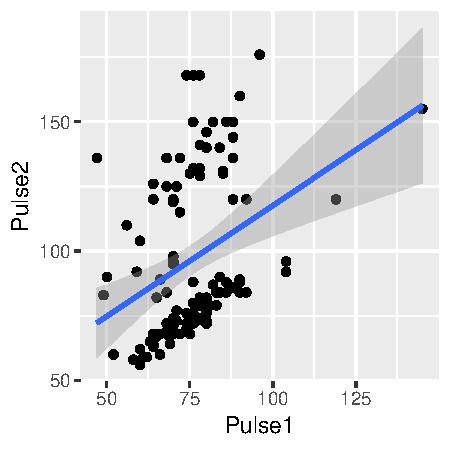
\includegraphics{seminar_060_tex_files/figure-latex/reg_plot-1} 

}

\caption{\label{fig:fig1} Регрессия пульса до упражнений на пульс после}\label{fig:reg_plot}
\end{figure}

Рисункки будут нумероваться отдельно от таблиц. Поэтому при ссылке на
Рисунок \ref{fig:reg_plot} мы увидим первый номер.

Упомянем наши источники, чтобы они появились в библиографии: Афанасьев и
Василевский (1992), Cobb (2011), Гультяев (2008), Doe и Pam (2011).

\section*{Библиография}
\addcontentsline{toc}{section}{Библиография}

\hypertarget{refs}{}
\hypertarget{ref-cobb2011teaching}{}
Cobb, George W. 2011. «Teaching statistics: Some important tensions».
\emph{Chilean Journal of Statistics} 2 (1): 31--62.

\hypertarget{ref-doe:website}{}
Doe, John, и Smith Pam. 2011. «the website title».

\hypertarget{ref-afanasyev92}{}
Афанасьев, В. В., и О. Н. Василевский. 1992. \emph{Расчеты электрических
цепей на программируемых микрокалькуляторах}. Москва: Энергоиздат.

\hypertarget{ref-microsoftProject2008}{}
Гультяев, А.К. 2008. \emph{Microsoft Office Project 2007 Professional.
Управление проектами: Практическое пособие.} СПб:.КОРОНА-Век.


\end{document}
